\chapter{Implementierung}

\begin{figure}[ftb]
\label{HauptAblauf}
\centering
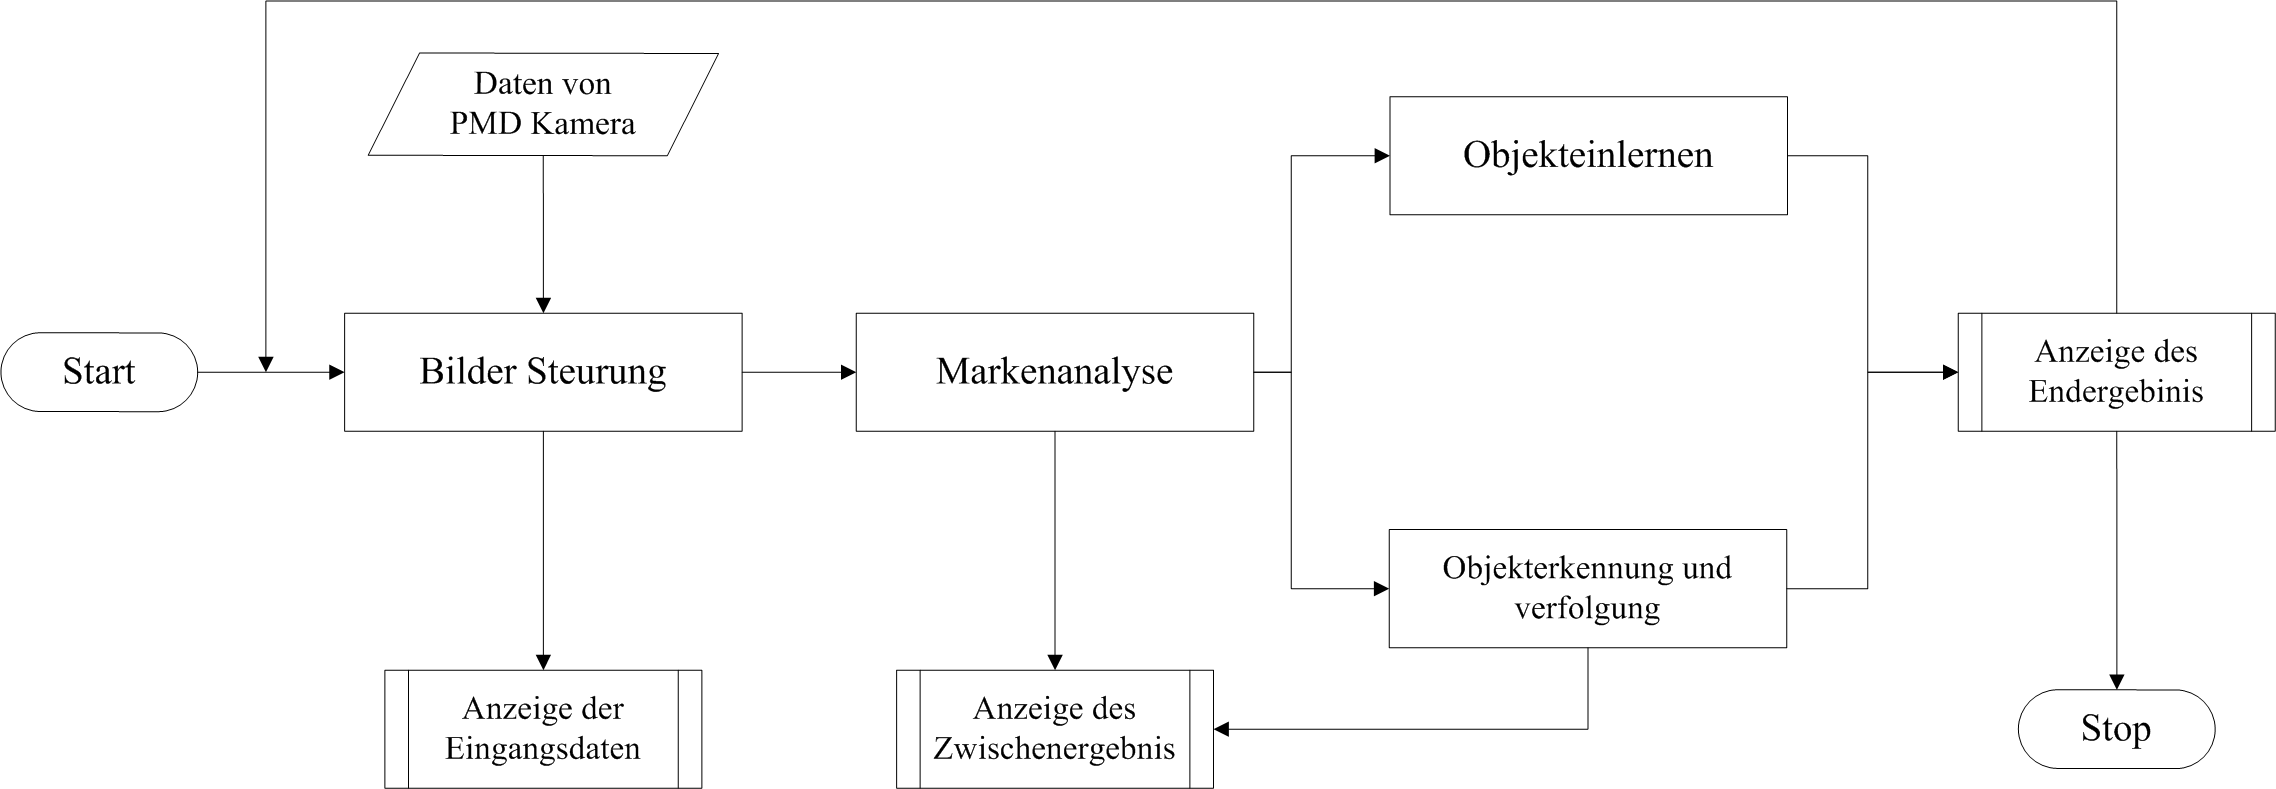
\includegraphics[scale=0.55]{Abbildungen/HauptAblauf.png}
\caption{Ablaufdiagramm}
\end{figure}

Unsere Implementierung kann in 4 Hauptmodule unterteilt werden:

\begin{itemize}
\item Markenanalyse
\item Objekteinlernen
\item Objekterkennung und Verfolgung
\item Bilder Steuerung
\end{itemize}

Die allgemeine Ablaufprozess des Programms findet man in Abbildung~\ref{HauptAblauf}. Das ganz Programm ist eine Schleife. In jedem Schritt wird die Information von PMD Kamera angesammelt und als Eingabe eingegeben. Nach Bewertung der neuen Eingabe bzw. der R�ckkopplung von letztem Ablauf wird die entsprechende Bilddaten von Modul Bilder Steuerung f�r die weiteren Schritten ausgew�hlt. Der Modul Markenanalyse analysiert die eingegebene Bilddaten und versucht die Marken zu finden und zu verfolgen. Die ausgefundene Marken werden von entweder dem Objekteinlernen oder der Objekterkennung und Verfolgen benutzt, welche am Anfang des Programms durch Benutzer entschieden wird. In der Einlernensphase wird zuerst die Transformation des Objekts bestimmt und dann das charakteristische Graph des Objekts durch die Marken dargestellt. Wenn man ein Objekt wieder erkennen m�chte, werden die Marken von neuem Objekt zu den vorhandenen charakteristischen Graphen verglichen, die nach dem Objekteinlernen im Speicher gespeichert werden. Das Ergebnis wird in einem OpenGL Fenster ausgemalt und au�erdem,  als die R�ckkopplung f�r den n�chsten Schritt zur�ck zum Anfang der Schleife geschickt. Alle diese Module werden in folgenden Unterabschnitten genau erkl�ren und ein ausf�hrliches Ablaufdiagramm wird in Abbildung~\ref{GenauAblauf} gezeigt.   

\begin{figure}
\label{GenauAblauf}
\centering
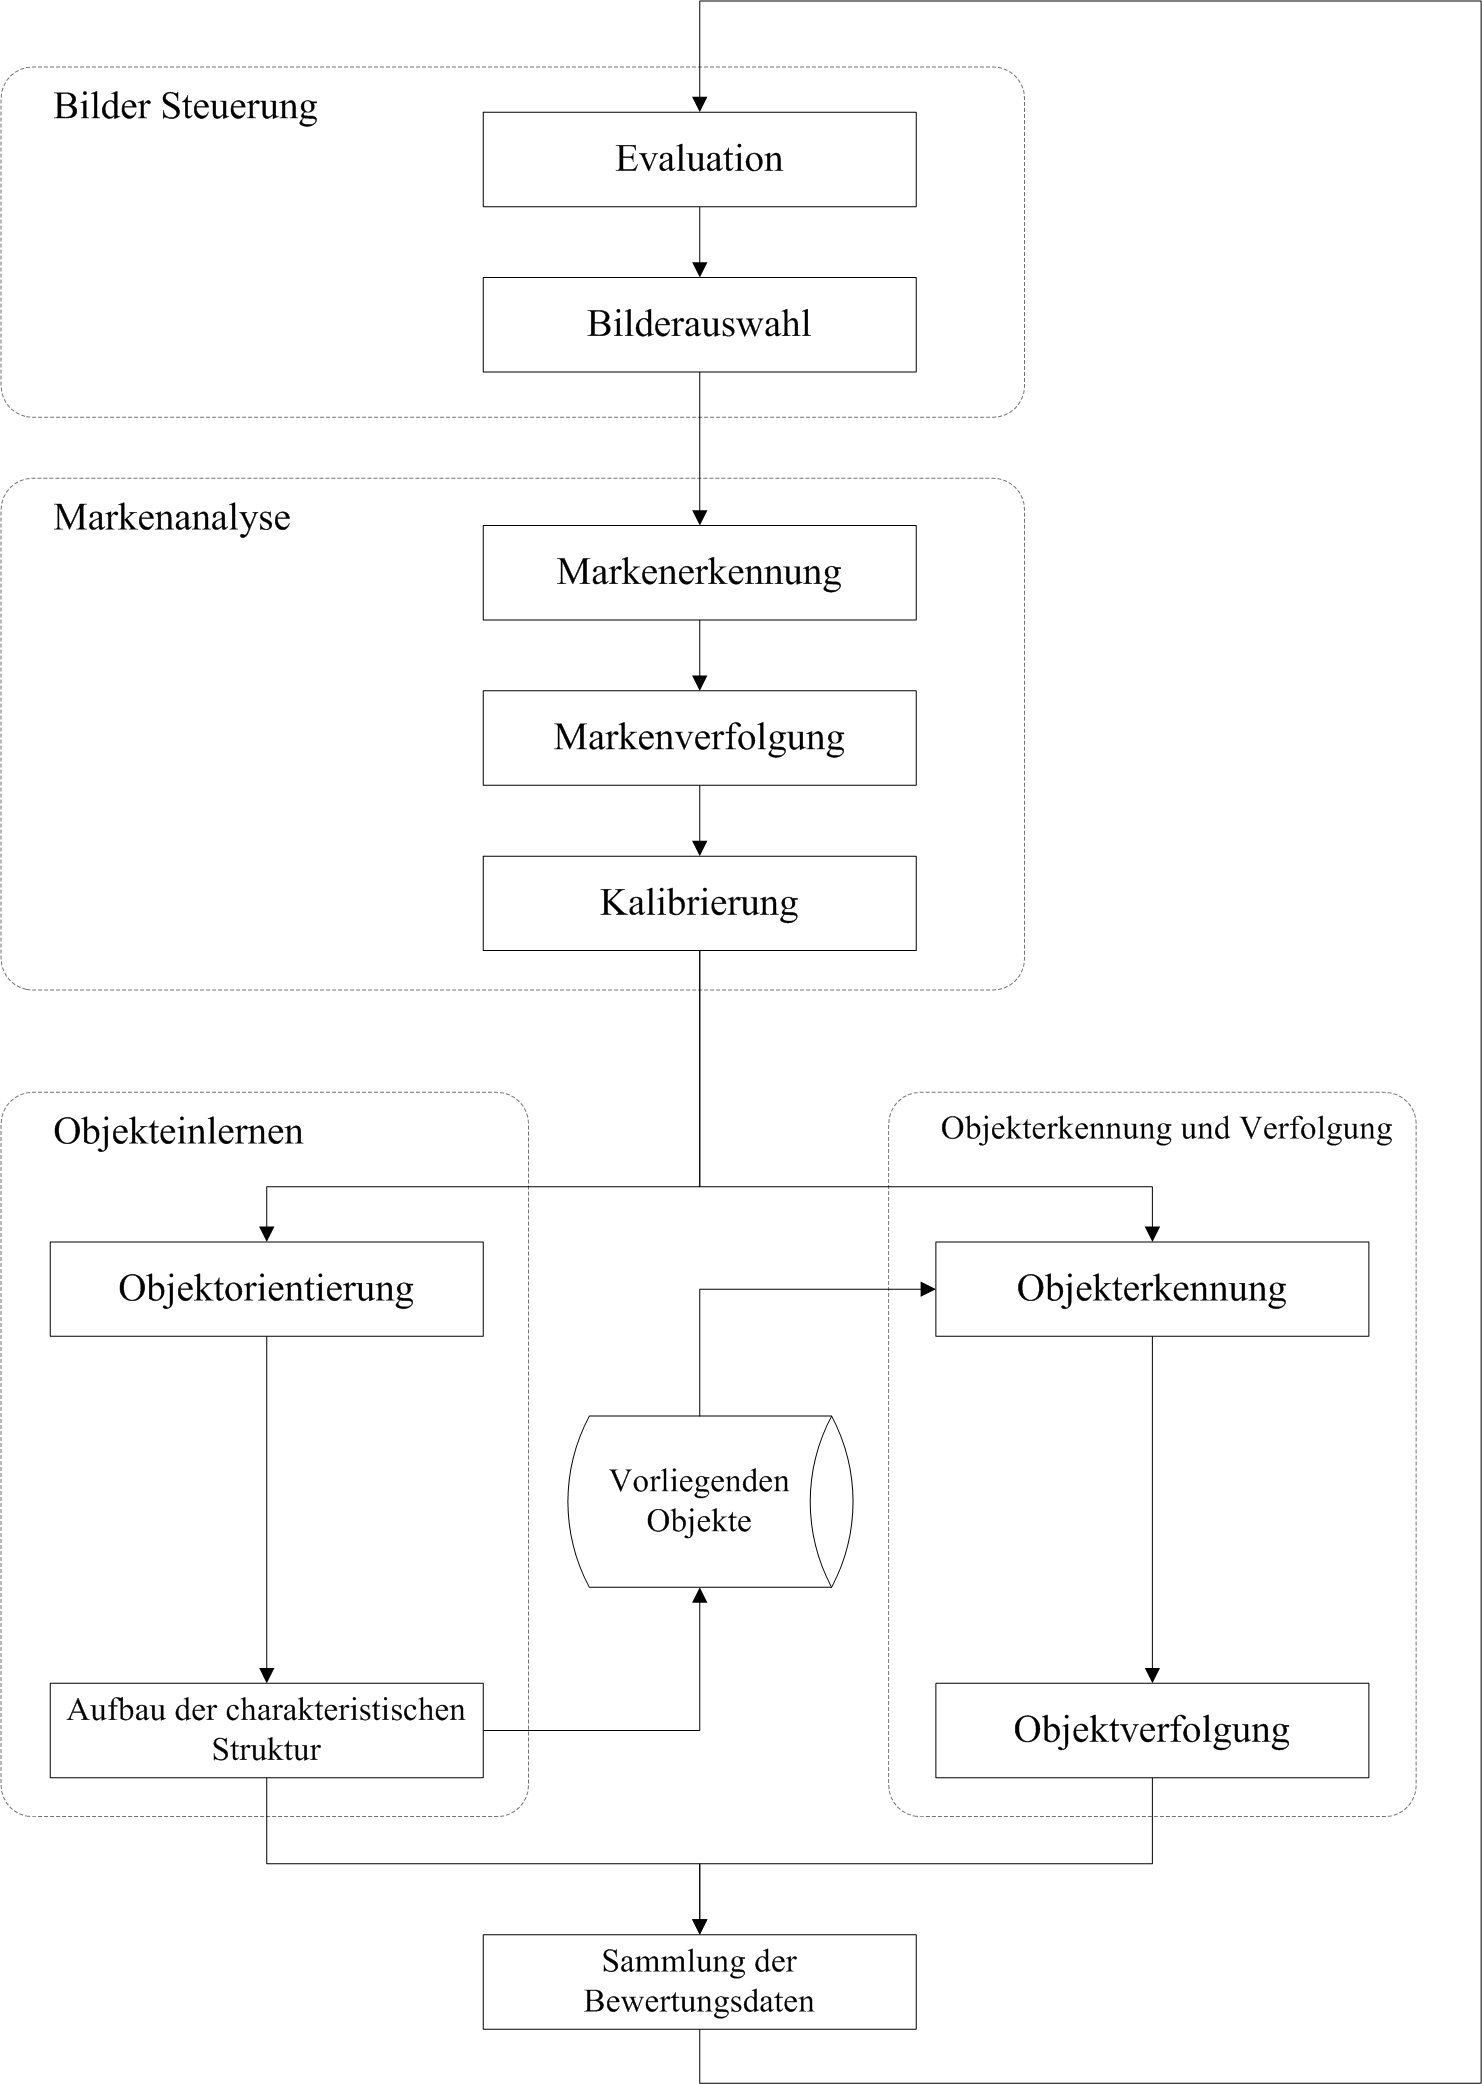
\includegraphics[scale=0.7]{Abbildungen/Ablaufsbild.png}
\caption{Ausf�hrliches Ablaufdiagramm}
\end{figure}

\section{Markenanalyse}

\subsection{Markenerkennung}

\subsubsection{Auswahl des Erkennungsalgorithmus}

\subsubsection{Auswahl der Gr��e der Marken}

\subsubsection{Kontrolle der Helligkeit}

\subsection{Markenverfolgung}

\section{Objekteinlernen}

\subsection{Markenanordnung}

\section{Objekterkennung und Verfolgung}

\section{Bilder Steuerung}